\documentclass[11pt,a4paper]{article}
\usepackage{fontspec}
\setmainfont{TeX Gyre Pagella}
\newfontfamily\headfont{Inter}[UprightFont=*-ExtraBold,BoldFont=*-ExtraBold,Extension=.otf,Path=/usr/share/fonts/opentype/inter/]
\usepackage[a4paper,margin=2.3cm]{geometry}
\usepackage{graphicx,booktabs,float,caption,array,xcolor}
\usepackage[hidelinks]{hyperref}
\usepackage{titlesec}
\usepackage[round]{natbib}
\usepackage{setspace}
\setstretch{1.05}
\renewcommand{\topfraction}{0.9}
\renewcommand{\bottomfraction}{0.8}
\renewcommand{\textfraction}{0.1}
\renewcommand{\floatpagefraction}{0.75}
\setlength{\parindent}{0pt}
\setlength{\parskip}{0.55em}
\titleformat{\section}{\headfont\Large}{\thesection}{0.8em}{}
\titleformat{\subsection}{\headfont\large}{\thesubsection}{0.8em}{}
\captionsetup{font=small,labelfont=bf}
\urlstyle{same}
\hypersetup{pdftitle={Who Held the Map? Twelve Centuries of the World in Flags},pdfauthor={Tristan Hotham}}

\begin{document}
\begin{center}
{\Large\bfseries Who Held the Map?\par}
\vspace{0.4em}
{\large Twelve centuries of the world in flags, 800 to 2010,\\from historical basemaps and Wikidata\par}
\vspace{1.2em}
{\large Tristan Hotham\par}
\vspace{0.3em}
{\small Independent researcher\\
ORCID: 0000-0003-4931-9349\\
DOI: \href{https://doi.org/10.5281/zenodo.23845995}{https://doi.org/10.5281/zenodo.23845995}\par}
\vspace{0.8em}
2026
\end{center}

\begin{quote}
\small
\begin{center}\textbf{Abstract}\end{center}
I combine the open historical-basemaps world maps \citep{ourednik} with flag and coat of arms statements in Wikidata to draw the world map at 30 dates from 800 to 2010, with each area filled with the flag of whoever held it at that date. The central problem is when not to show a flag: most polities flew no national flag before about 1700, many basemap areas are peoples or cultural regions rather than states, and Wikidata labels are ambiguous. I set out explicit rules: a flag is shown only when a Wikidata statement, dated by qualifiers or by the image's file name, covers the year, or when an undated flag belongs to a historical state within its lifetime and after 1150; otherwise a coat of arms, a plain colour, or a neutral style for peoples. Of 680 states, 535 (78.7\%) matched a Wikidata item, covering 94.2\% of the land they held. The share of the world's land that can honestly be filled with a flag in use rises from zero in 1000 and 3.7\% in 1500 to 74.8\% in 1900 and 97.3\% in 2010. The largest single entry in the basemap is the Mongol Empire in 1279 (20.5\% of the world's land); counting only the United Kingdom and its self-governing dominions, the British Empire in 1914 was larger (24.1\%). European states held 4.9\% of the land in 1492 and 46.1\% in 1914, Russia included. For 93 of 194 present-day countries Wikidata dates the current flag; the median start year is 1986, often a re-specification rather than a new design. The results describe the basemaps and Wikidata as much as history, and I report their limits throughout.

\textbf{Keywords:} flags; vexillology; historical maps; empires; colonialism; Wikidata; historical GIS; open data
\end{quote}

\section{Introduction}
World maps filled with national flags are a popular image. They imply a question that is harder than it looks: what would the same map have looked like in 1500, or 1000? Answering it needs two things, a map of who held each piece of land at a date, and a record of which flag each holder used at that date. Both exist in open form. The historical-basemaps project \citep{ourednik} provides world maps for many dates, naming each area and the power controlling it. Wikidata \citep{wikidata} records the flags (property P41) and coats of arms (P94) of many states, often with start and end dates, and Wikimedia Commons holds the images.

This paper joins them, with an interactive companion (\url{https://maps.tristanhotham.com/flags-through-time/}) whose time slider steps through the snapshots. Its contribution is less the picture than the rules: a transparent procedure for deciding, area by area and date by date, whether a flag can be shown without anachronism, and an account of what the result says and does not say. It also reports four summaries: the share of land that can be shown with a flag, the largest holders of land, the share held by European states and their empires, and the age of today's flags.

\section{Data}
\subsection{Historical basemaps}
historical-basemaps \citep{ourednik} is a set of GeoJSON world maps, released under GPL-3.0, for dates from 123{,}000 BC to 2010. Each polygon has a name (NAME), the power exercising authority over it (SUBJECTO; the area's own name otherwise), an optional larger cultural area (PARTOF) and a border precision from 1 (approximate) to 3 (determined by international law). I use the 30 dates from 800 to 2010. The maps are uneven in detail: the 1492 map names 1,177 peoples and cultural regions, 1,165 of them nations of the Americas, while other dates draw whole continents in a few blocks. The project's own documentation warns that the maps are work in progress, that boundaries before the modern period are often zones rather than lines, and that they should be checked against other sources for academic work.

\subsection{Wikidata and Commons}
For every name in the basemaps, a query on the QLever endpoint \citep{qlever} returned the Wikidata items with that English label or alias, with sitelink counts, inception and dissolution dates, flag statements with their start and end qualifiers, and coats of arms. Images are 160 pixel thumbnails from Wikimedia Commons; 413 are used (398 flags and 15 coats of arms), of which 357 are public domain or CC0 and 52 CC BY-SA. Each is credited with its source page and licence in the data. Two present-day flags missing from the downloaded set (the People's Republic of China and North Korea) were drawn from the flag-icons project \citep{flagicons}. Natural Earth \citep{naturalearth} supplies present-day countries for the flag-age analysis.

\section{Methods}
\subsection{Owners and land}
Each area's holder is its SUBJECTO, with spelling variants joined (for example USA, United States and United States of America) and a trailing colonial tag such as ``(UK)'' or ``(France)'' read as the holder. I corrected 2 labelling errors in the 1930 map (the Soviet Union's polygon labelled White Russia, and the Far Eastern Republic eight years after it joined Soviet Russia). Land is measured by rasterising each snapshot on a 0.1 degree grid weighted by the cosine of latitude, largest areas first so that enclaves win where polygons overlap, and leaving out Antarctica. Each snapshot holds about 133.0 million km$^2$ of land.

\subsection{Peoples, groups and states}
Holders are classed as peoples or cultural regions (names such as ``Bantu peoples'', ``Amazon hunter-gatherers'', ``Sámi'', and the nations of the Americas and Australia named in the detailed maps), loose groups of states (``minor Hindu kingdoms'', ``Chinese warlords''), or states. Of 2,523 holders, 680 are states, 1,809 peoples or regions and 34 groups. Peoples and groups never receive a flag: many of these societies governed themselves without states, none used a national flag of the European kind, and flags some use today would be anachronistic.

\subsection{Matching to Wikidata}
Labels are ambiguous. For each state and snapshot year I take the candidate items whose inception and dissolution (with 30 years' tolerance) cover the year, or that have no dates, and choose by sitelinks, a preference for English labels over aliases and the presence of a flag or arms. For 76 important holders I set the items by period by hand, for example the Kingdom of France before 1792 and France after, the Republic of China to 1949 and the People's Republic after, the Spanish Habsburg monarchy and Spain, and the Dutch Republic and the Netherlands.

\subsection{Choosing the emblem}
For a state in year $y$ I consider the flag statements of its items, excluding files described as fictitious, conjectural or unofficial, in this order:
\begin{enumerate}
\item a flag whose start and end (from qualifiers, else years in the file name written as a range of years) cover $y$; the latest start wins;
\item a flag with no dates, if the state no longer exists, $y$ falls within its inception and dissolution and $y \ge 1150$; for a present-day state, only from 1900 (or from the first start date recorded for the same image on any present-day country), with two documented exceptions, Denmark's flag from 1400 and Sweden's from 1600;
\item a coat of arms, for a historical state of under 400 years' life within its lifetime from 1150, or any arms whose file name dates cover $y$;
\item otherwise a plain colour with the name.
\end{enumerate}
The year 1150 marks the emergence of heraldry \citep{pastoureau}. Of 3,386 state-years, 1,412 (42\%\%) get a flag, 40 arms and 1,934 a plain colour; 42\%\% of flags rest on undated statements.

\subsection{Flag ages}
For present-day countries (Natural Earth sovereign countries) I take the open-ended P41 statement with the latest start date as the current flag, and bin the start years by 20-year period.

\section{Results}
\subsection{A map that fills with flags}
Figure~\ref{fig:mult} shows six snapshots and Figure~\ref{fig:cover} the share of land by emblem. In 1000 no land can be shown with a flag in use; 48\%\% belonged to peoples and cultural regions and 25.2\% has no holder named. Banners appear from 1200, led by the Holy Roman Empire and Venice (Figure~\ref{fig:eur}), but the share is only 3.7\% in 1500 and 40.9\% in 1800. It passes half in 1878 and reaches 97.3\% in 2010. The dip in 1920 is the Soviet state, whose first recorded flag dates from 1922.

\begin{figure}[tbp]\centering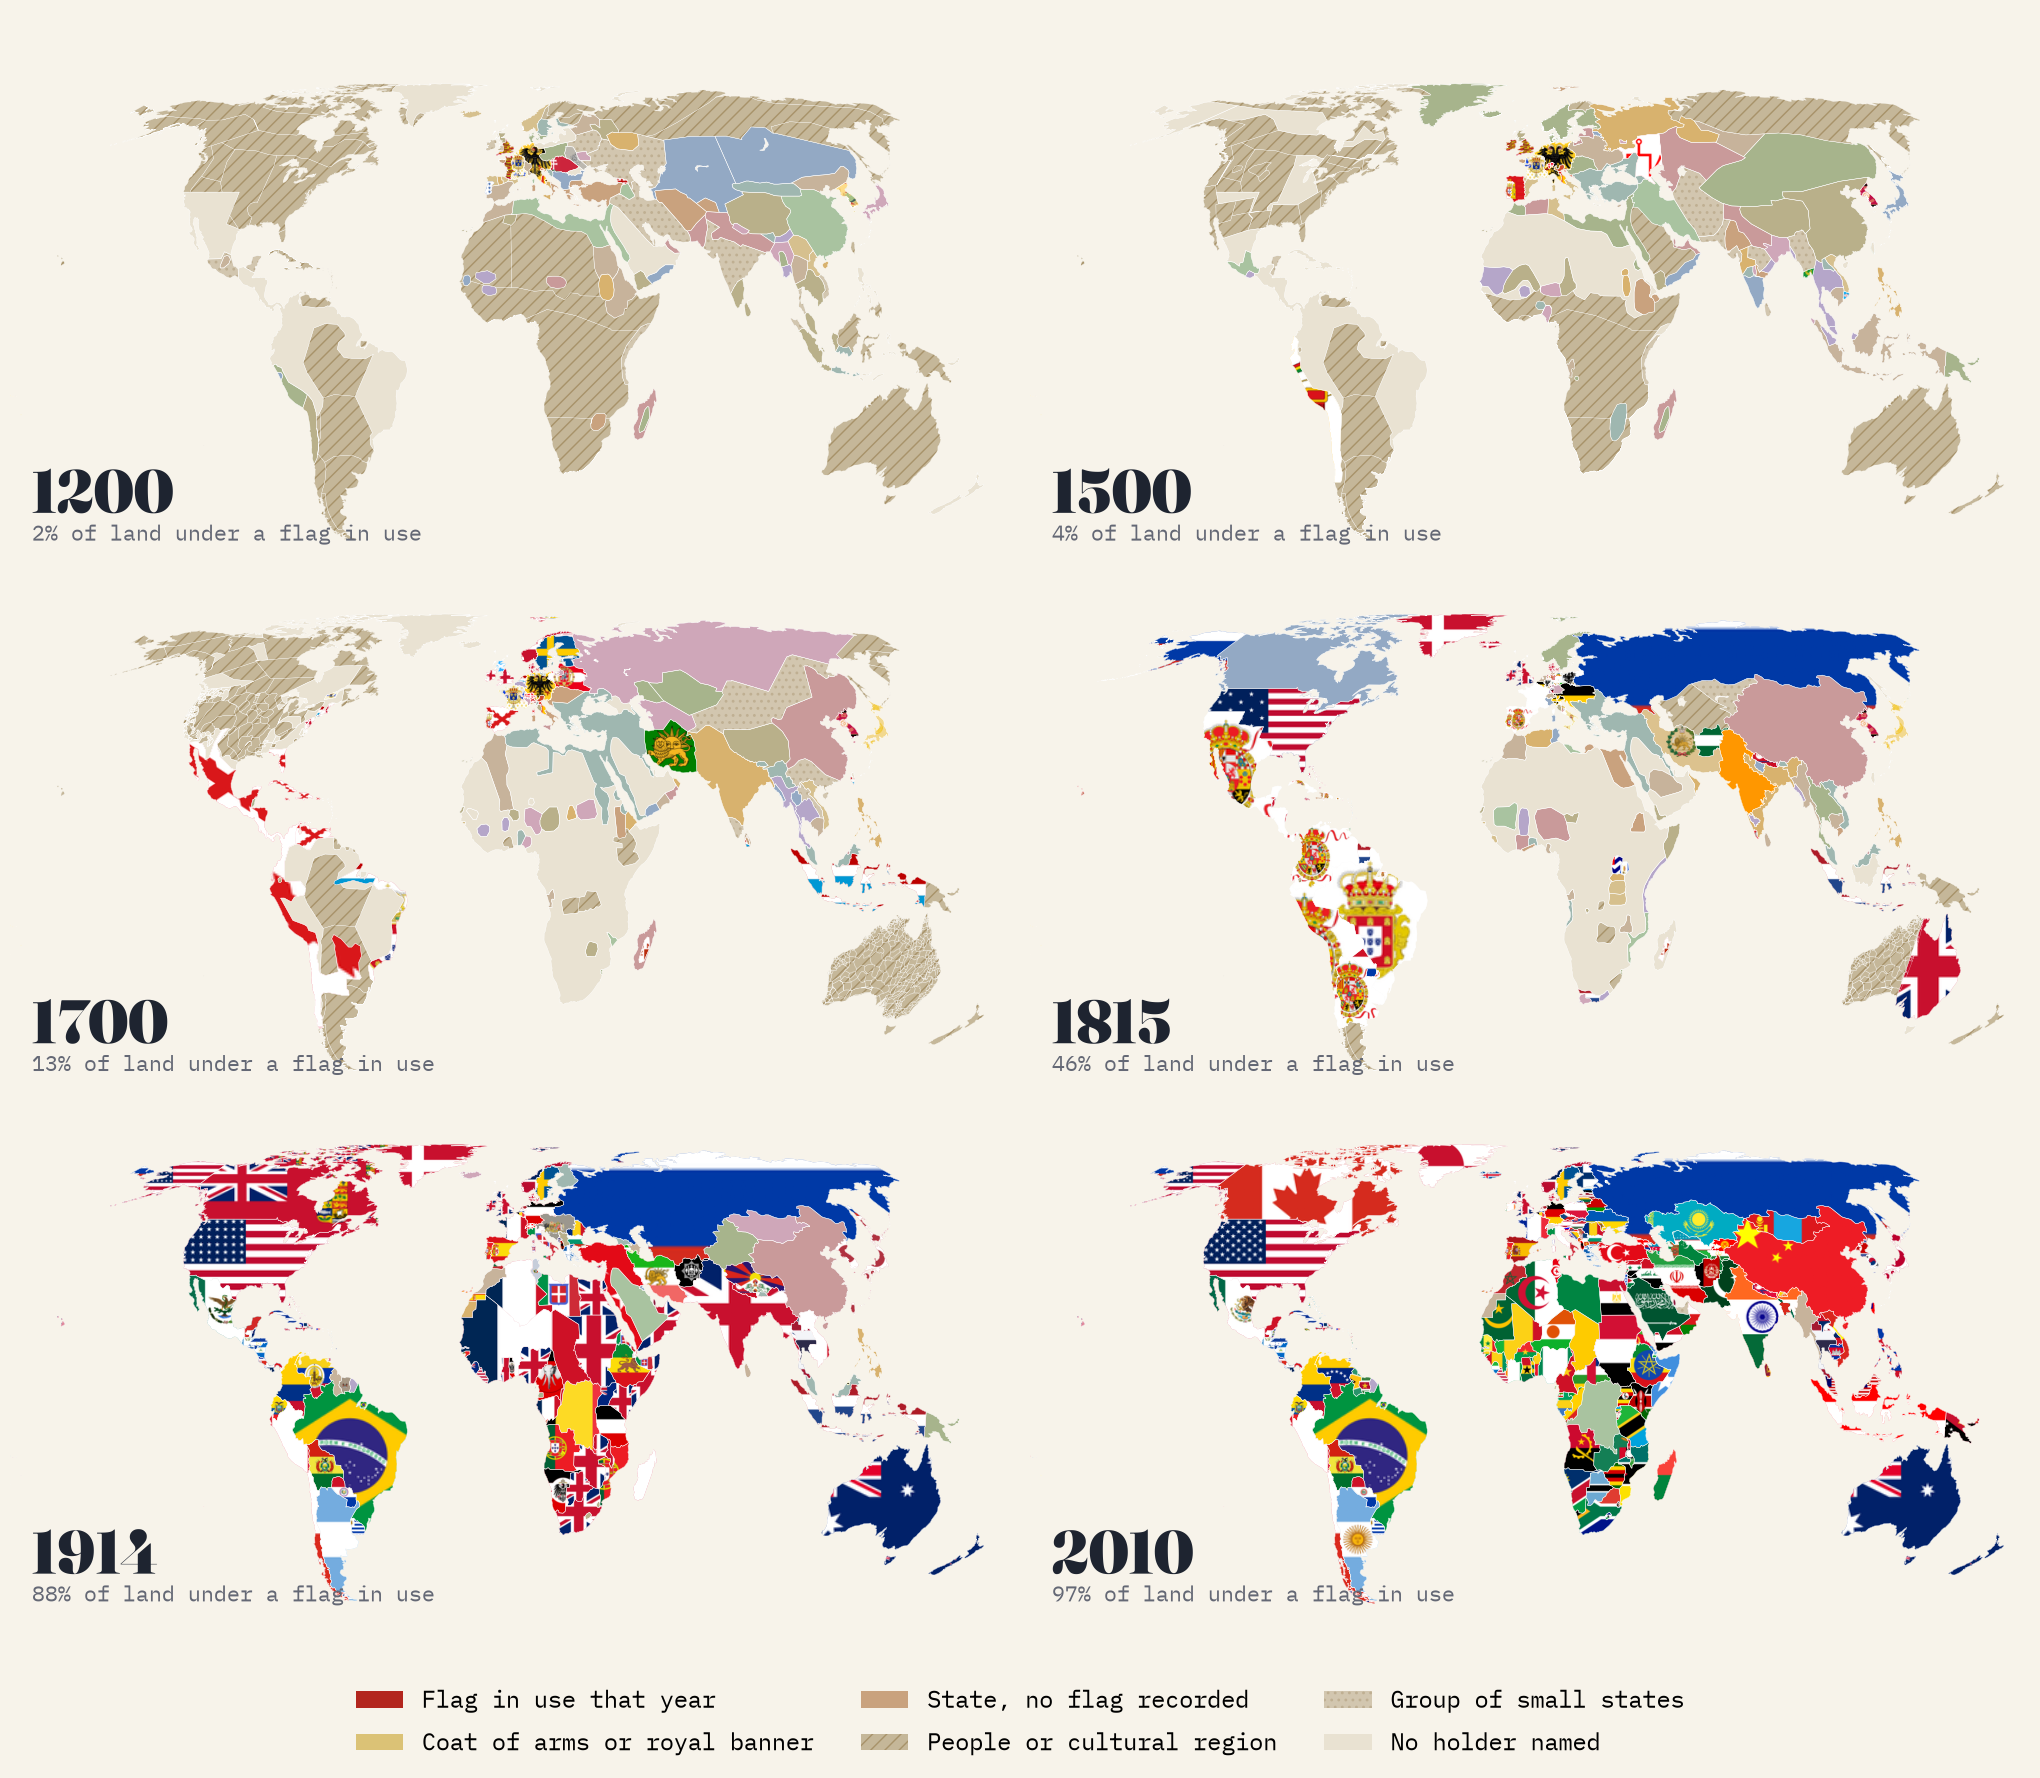
\includegraphics[width=\textwidth]{f_multiples.png}
\caption{The world in flags at six dates. Each area is filled with the flag of its holder when a flag in use that year is recorded.}\label{fig:mult}\end{figure}

\begin{figure}[tbp]\centering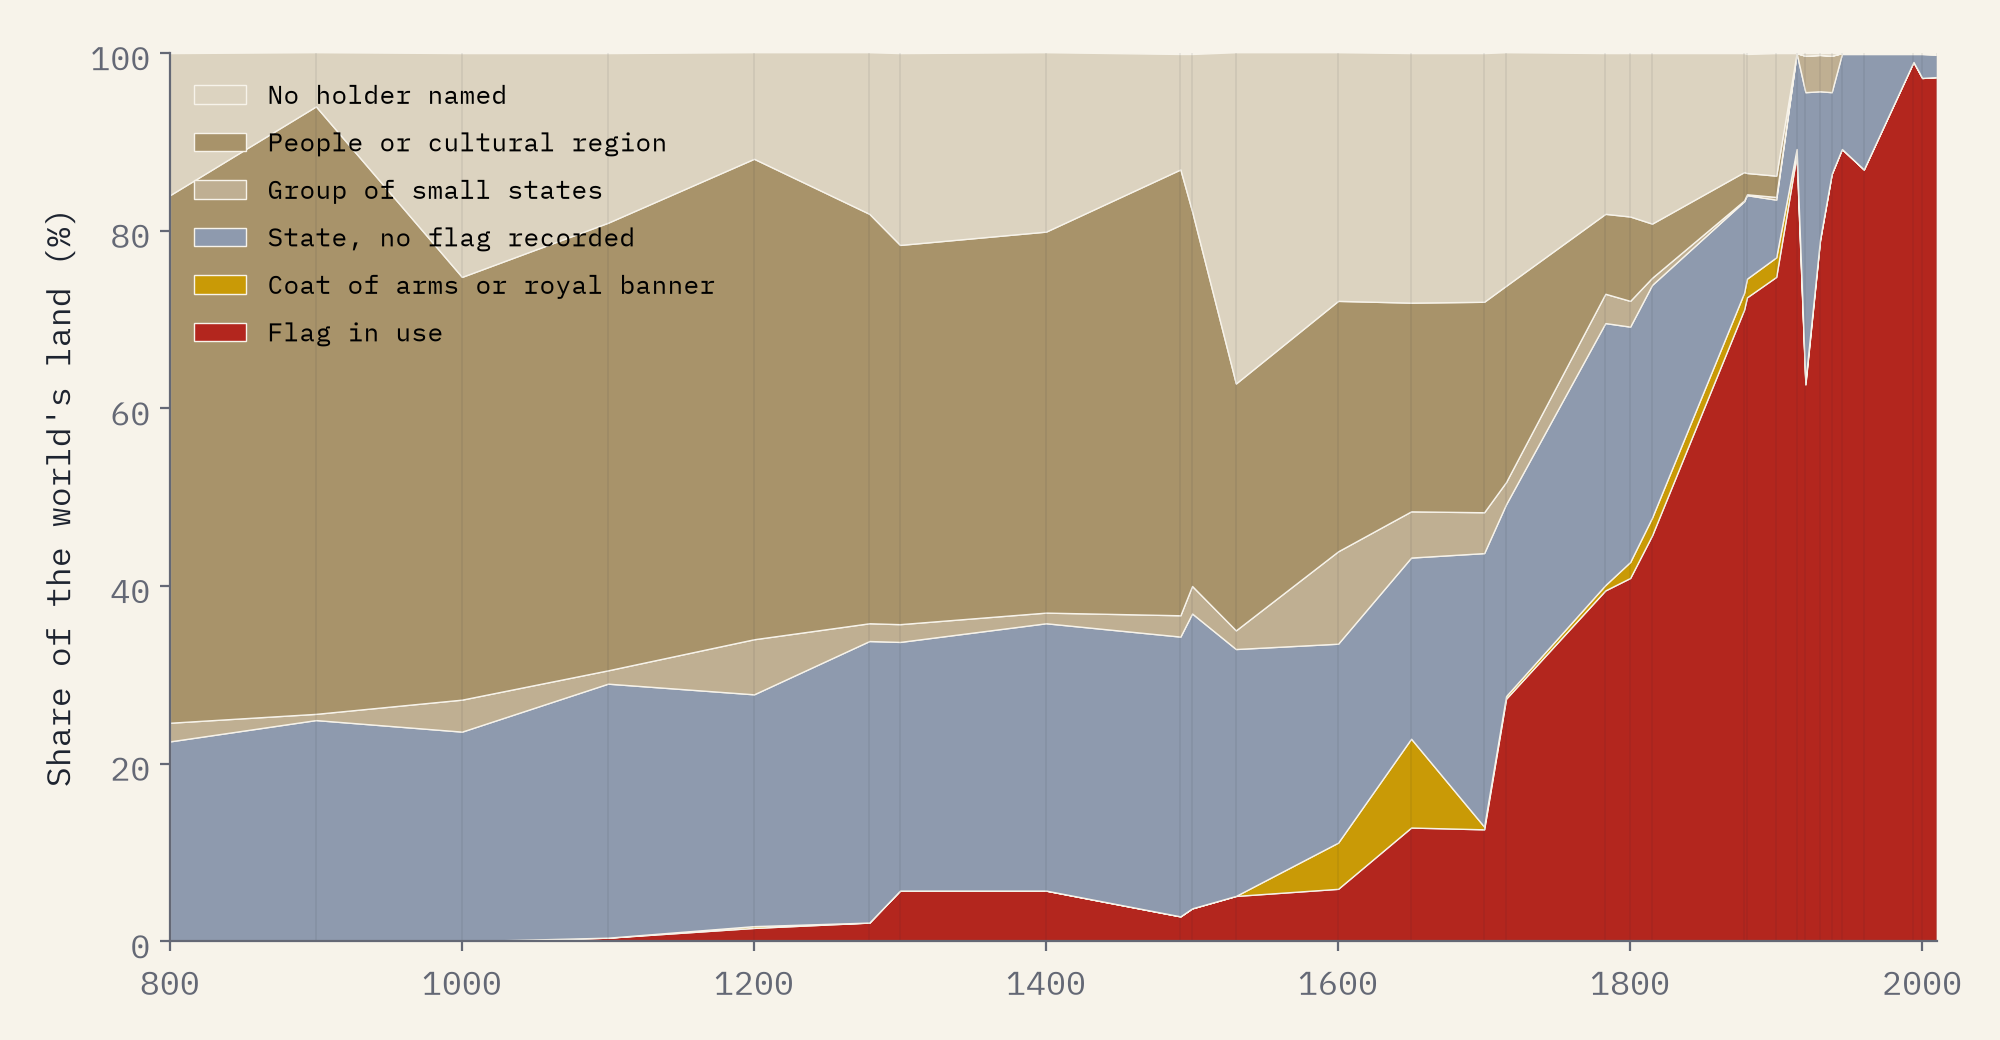
\includegraphics[width=.86\textwidth]{f_cover.png}
\caption{Share of the world's land (Antarctica excluded) by the emblem shown, at each snapshot.}\label{fig:cover}\end{figure}

\begin{figure}[tbp]\centering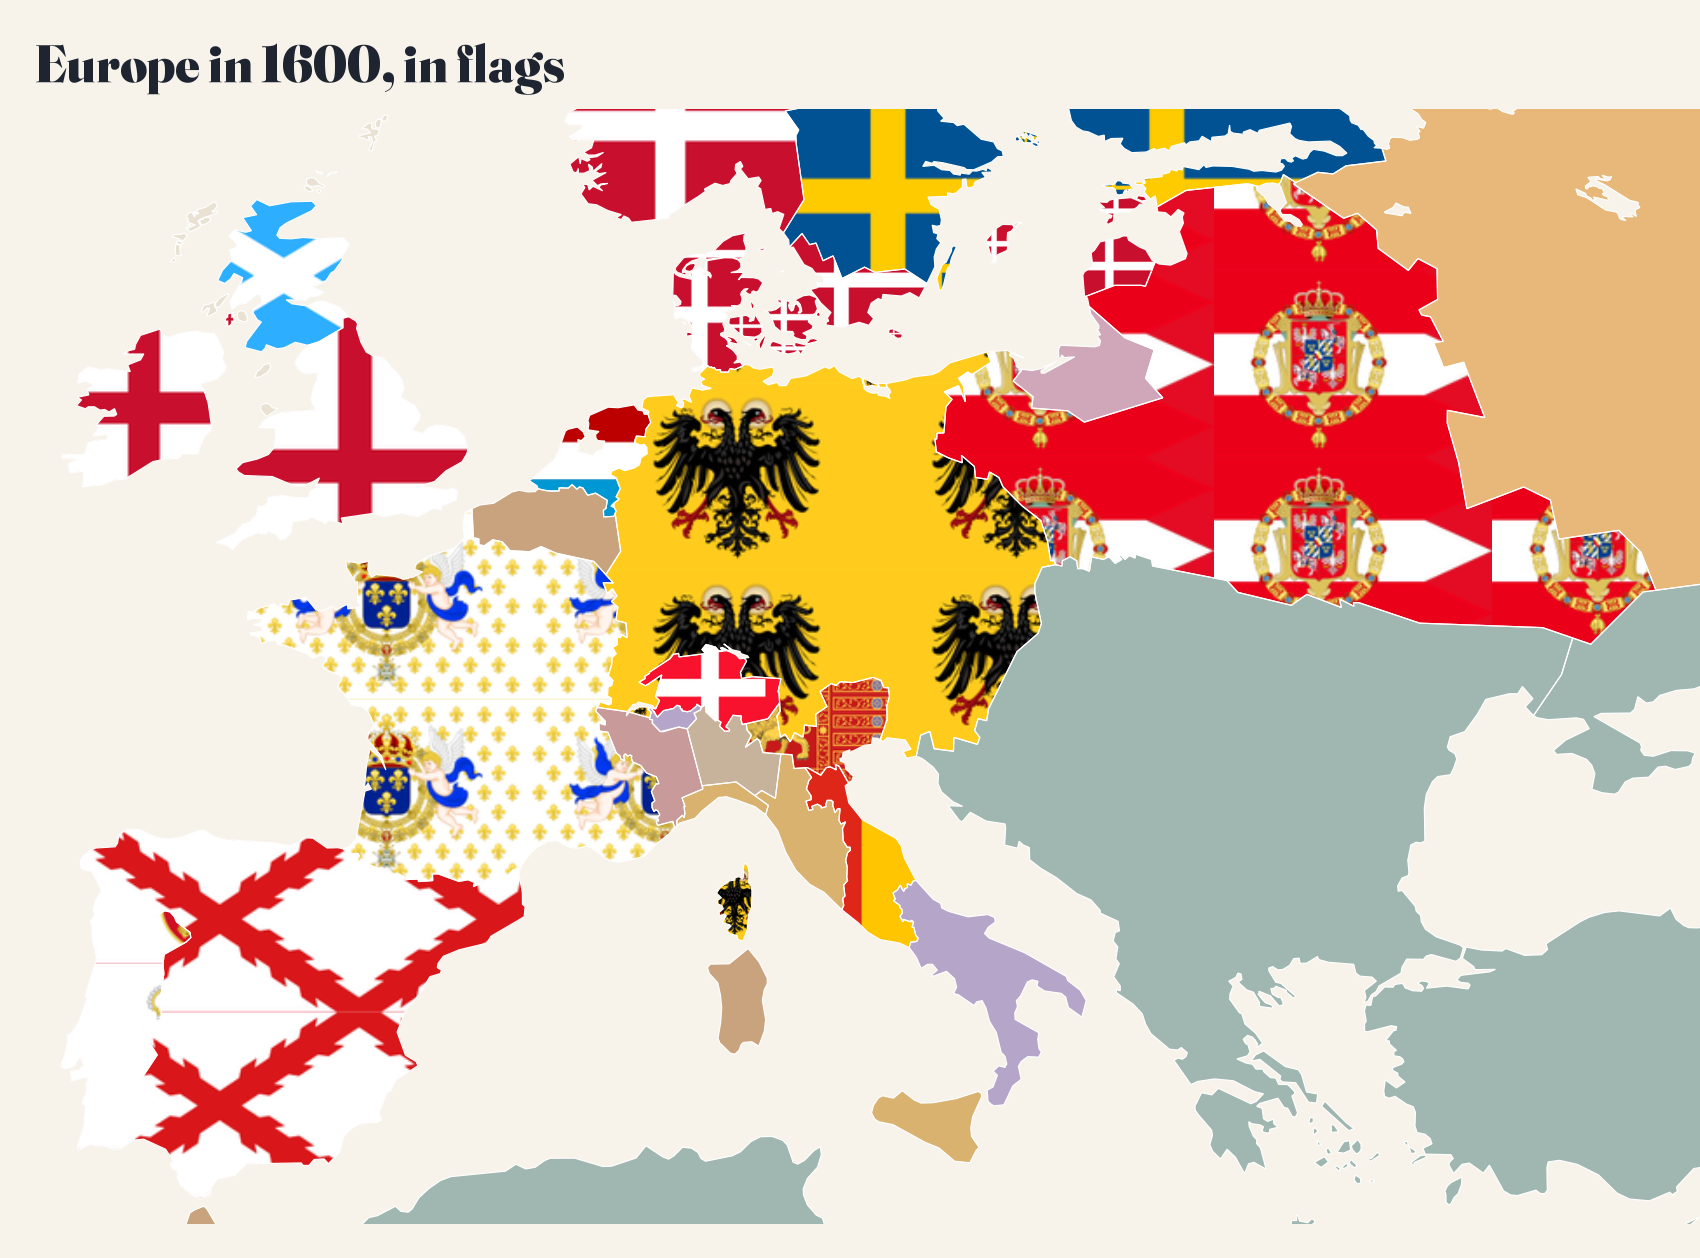
\includegraphics[width=.86\textwidth]{f_europe1600.png}
\caption{Europe in 1600: royal banners, crosses and arms. The Ottoman Empire has no flag in Wikidata for that year and is plain.}\label{fig:eur}\end{figure}

\subsection{The largest holders}
The largest single entry in the basemap at any date is the Mongol Empire in 1279, with 27.3 million km$^2$ (20.5\%; Figure~\ref{fig:big}), the largest contiguous land empire on the map. It is not the largest empire overall: counting only the United Kingdom and its self-governing dominions, the British Empire in 1914 held 24.1\%. From 1600 the largest single entry in every snapshot is Russia under one name or another, reaching 22.1 million km$^2$ in 1945. The Qing Empire peaked at 9.2\% in 1800. Land the basemap assigns to the United Kingdom peaks at 11.0\% in 1914; with the dominions it is 24.1\%.

\begin{figure}[tbp]\centering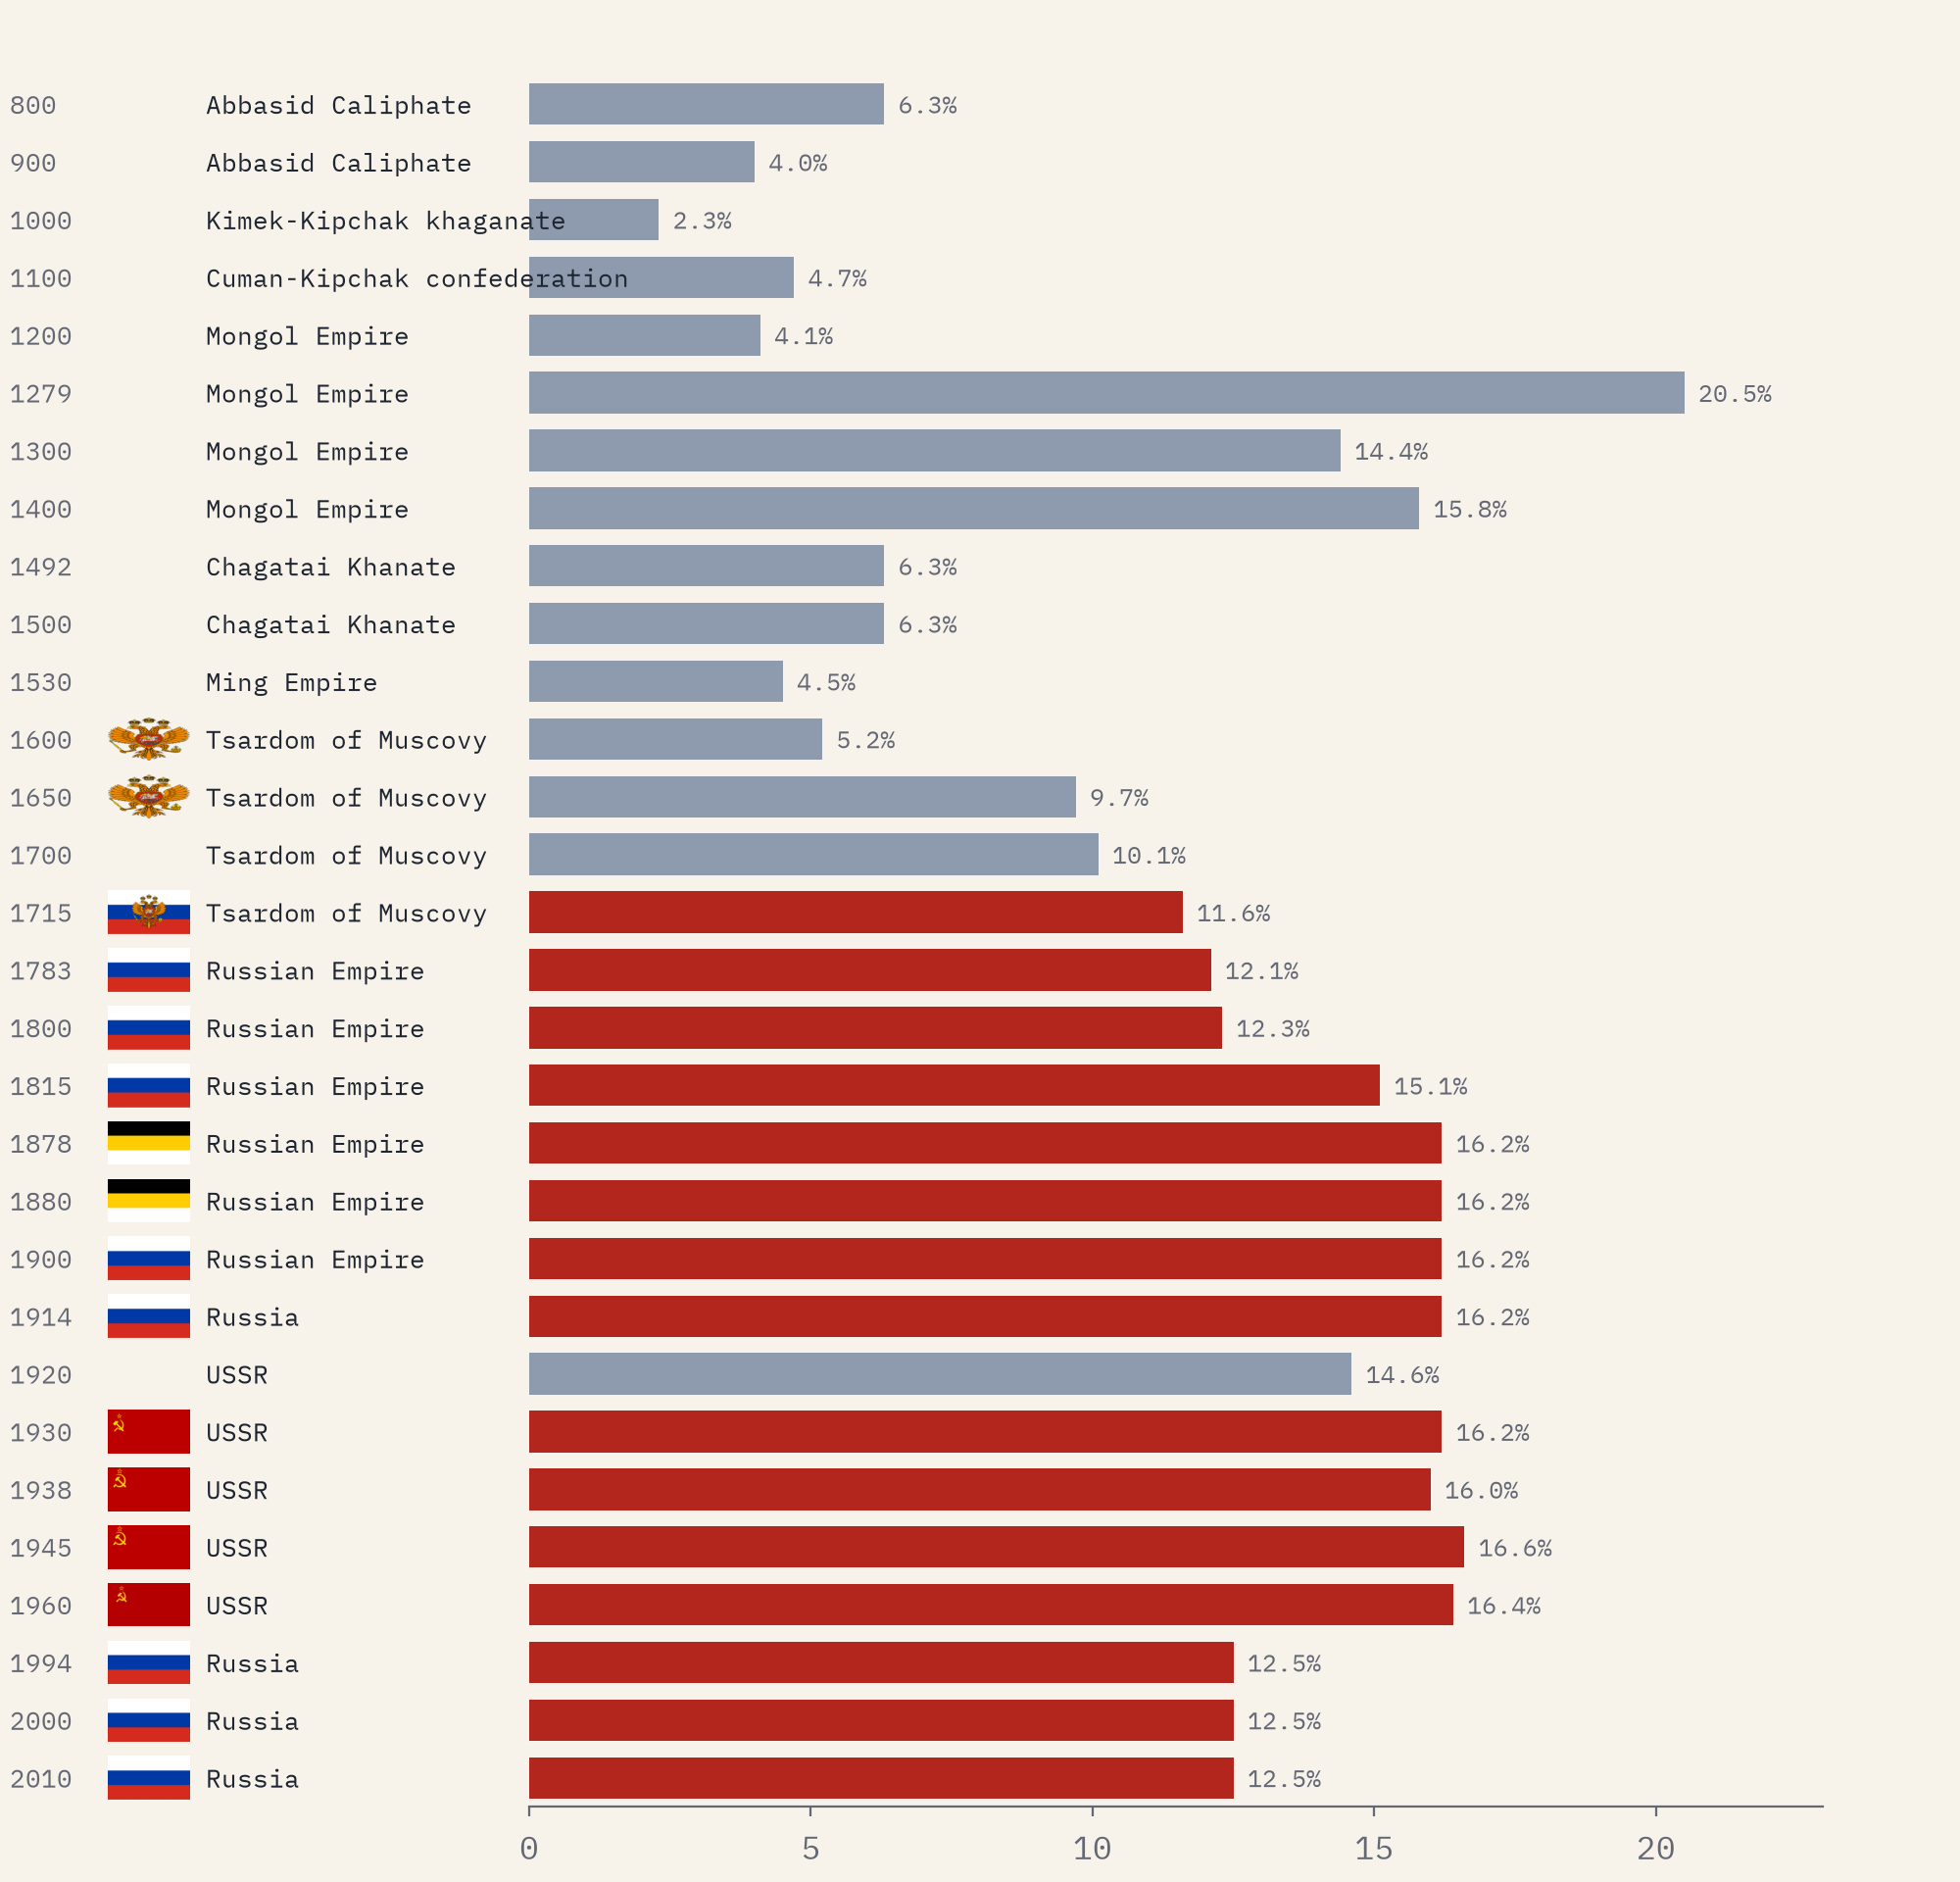
\includegraphics[width=.8\textwidth]{f_largest.png}
\caption{The largest holder of land at each snapshot, with its emblem where one is shown.}\label{fig:big}\end{figure}

\subsection{European empires}
European states held 4.9\% of the land in 1492 and 46.1\% in 1914: 27.3\% outside Europe, 16.2\% in the Russian Empire and 2.6\% in Europe (Figure~\ref{fig:euro}). Without Russia the peak is 29.9\% (1914). The fall from 1815 to 1878 reflects Latin American independence. The low values in 1960 are partly an artefact of the basemap, which draws most colonies as their own countries in that snapshot; in 1920 and 1930, areas held by a European power in both 1914 and 1938 but labelled as their own make up 1.2\% of the land.

\begin{figure}[tbp]\centering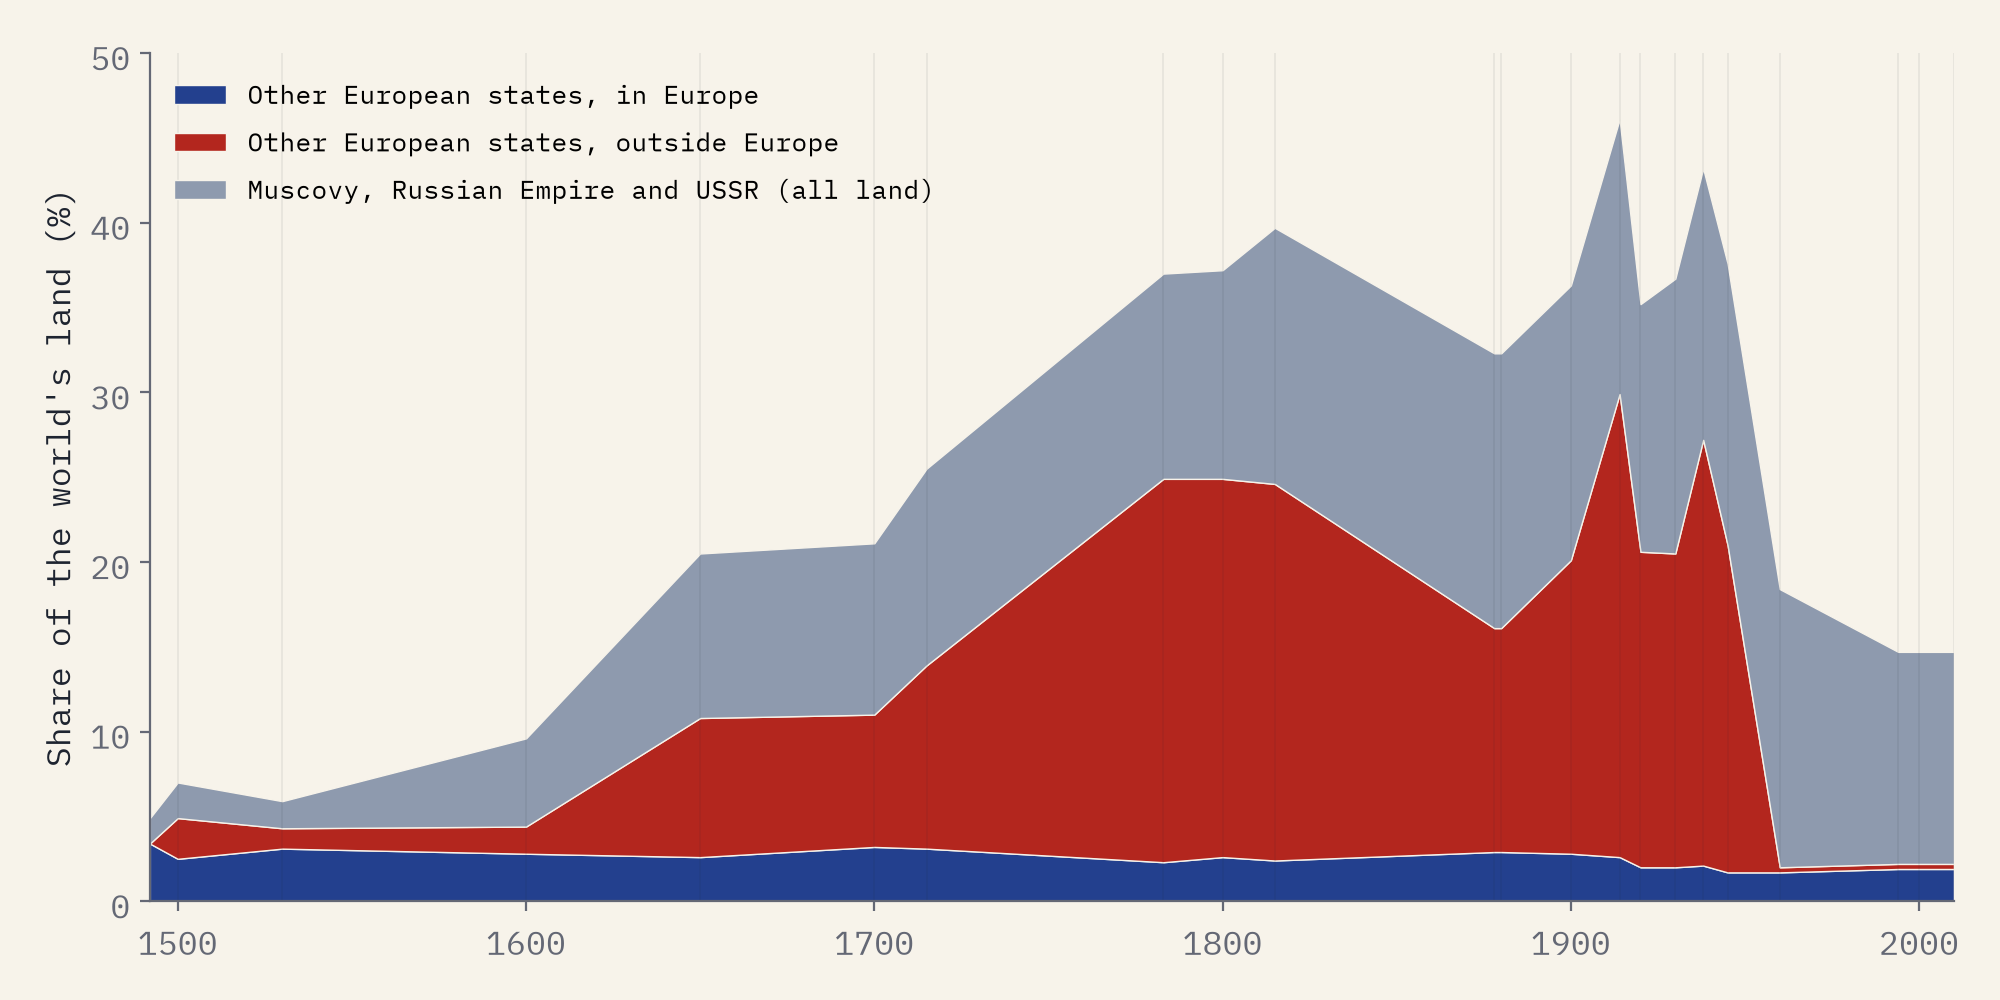
\includegraphics[width=.86\textwidth]{f_euro.png}
\caption{Share of the world's land held by European states, 1492 to 2010.}\label{fig:euro}\end{figure}

\subsection{Places through time}
Following single points gives each place a sequence of holders (Figure~\ref{fig:cities}). Moscow has the most among sixteen cities (9). Beijing passes from the Tang to the Liao, the Mongols, the Ming, the Qing, the warlords and China, shown with the Republic of China's flag in 1945 and the People's Republic's from 1960.

\begin{figure}[tbp]\centering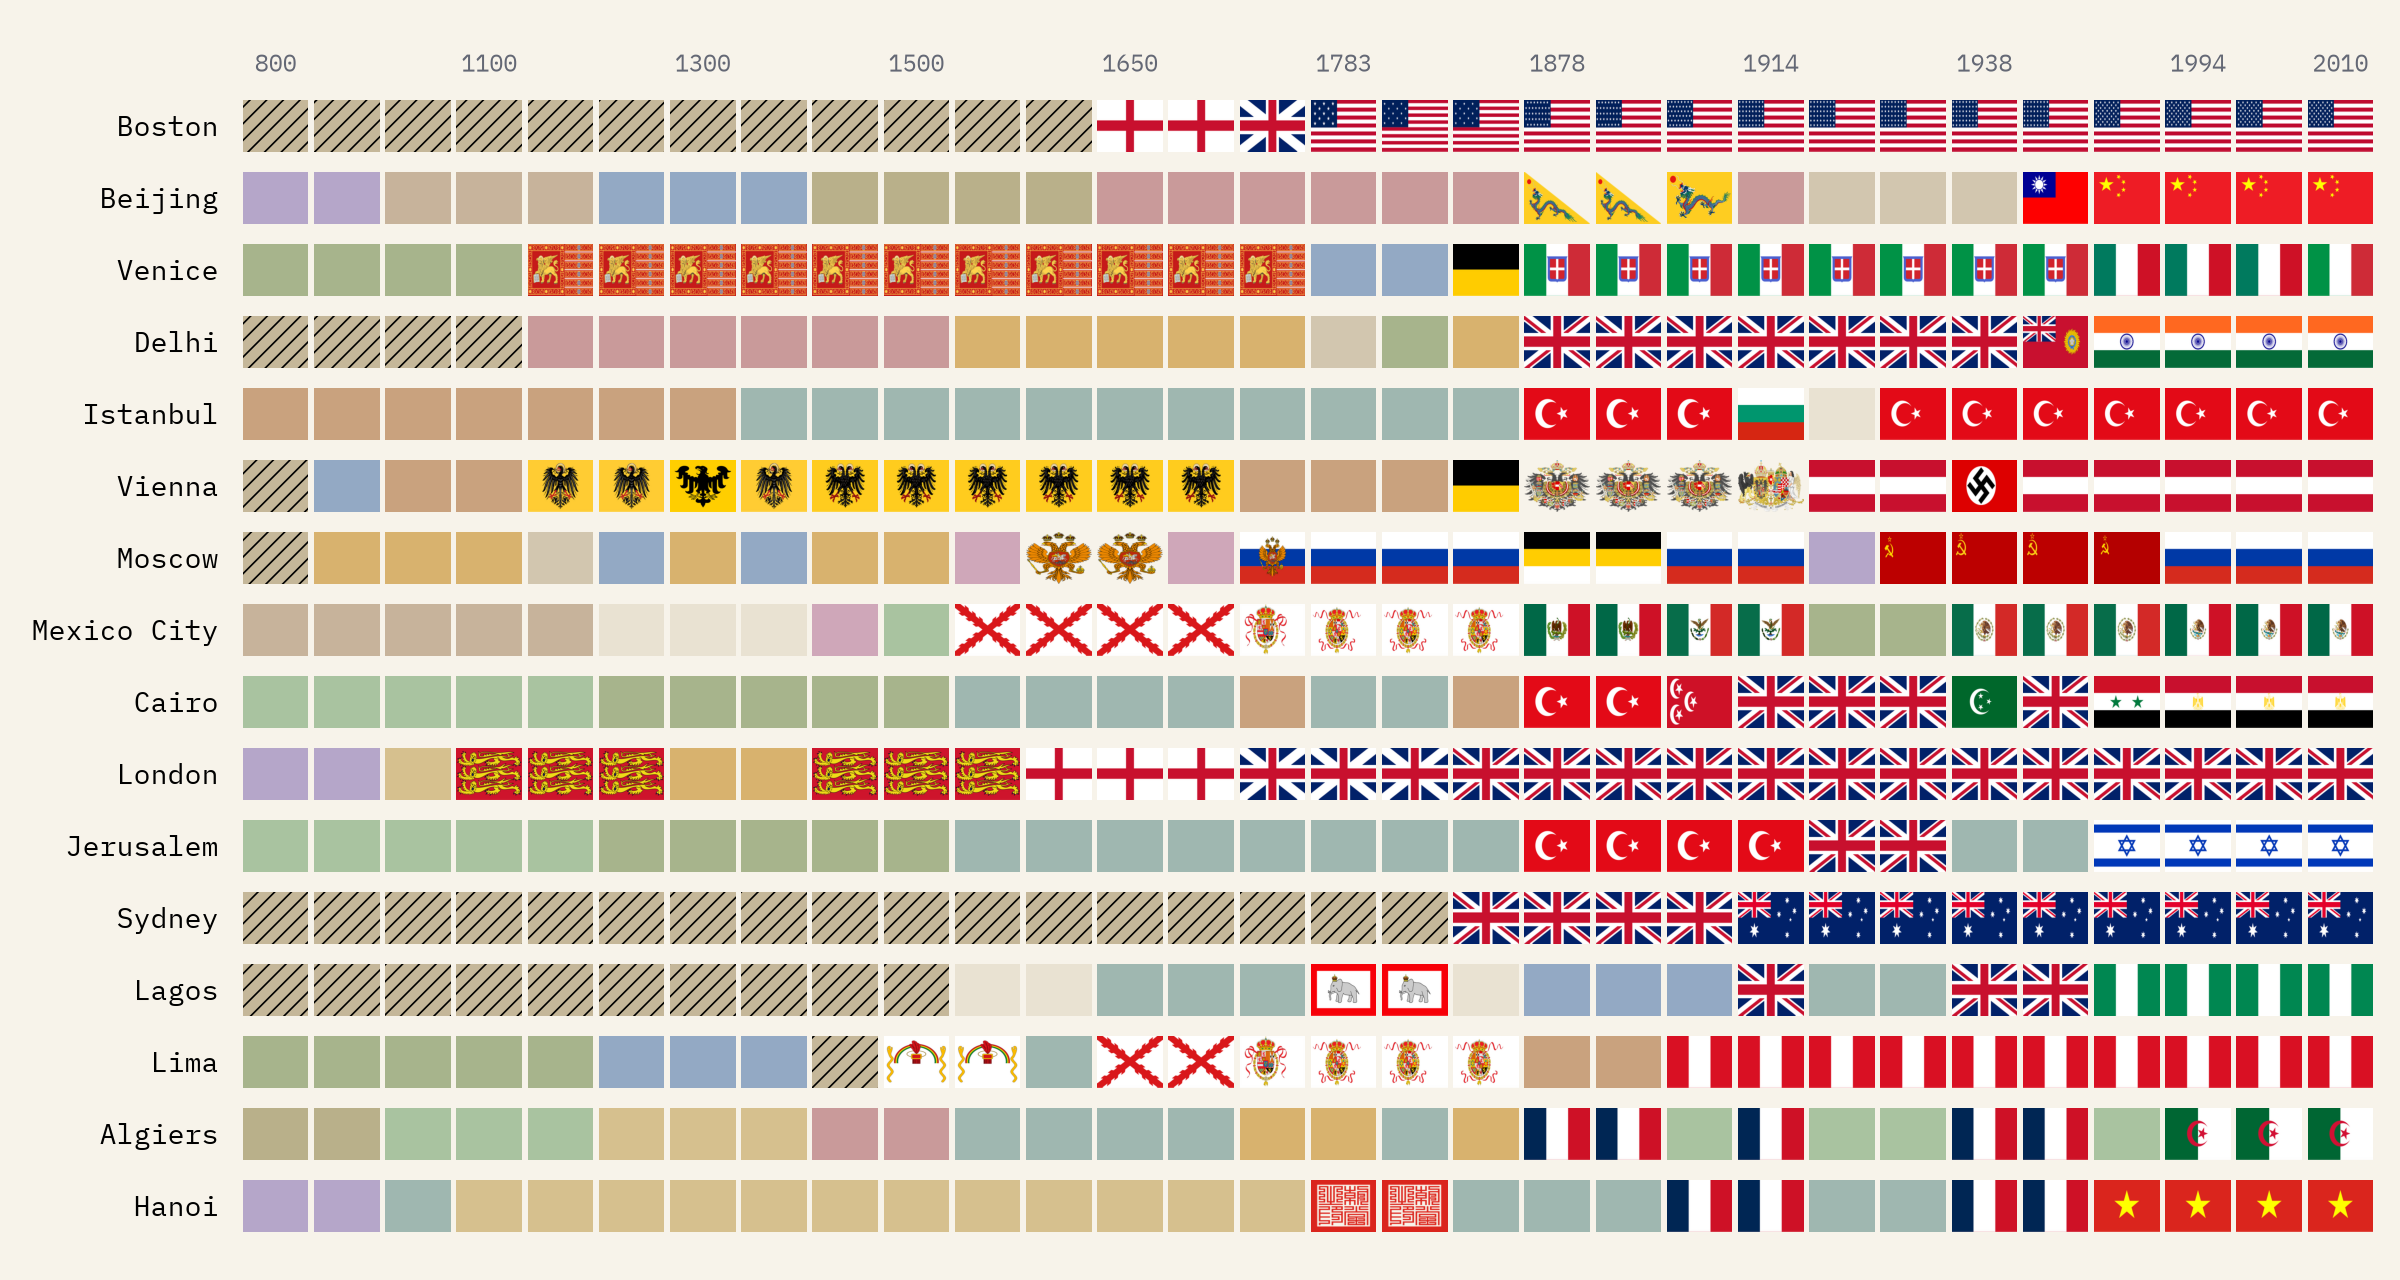
\includegraphics[width=\textwidth]{f_cities.png}
\caption{Holders of sixteen cities at each snapshot, shown by their emblem; hatched cells are peoples or cultural regions.}\label{fig:cities}\end{figure}

\subsection{Counting states}
The number of states per snapshot ranges from 58 (800) to 187 (1994) (Figure~\ref{fig:states}), but it tracks the level of detail of each map as much as history.

\begin{figure}[tbp]\centering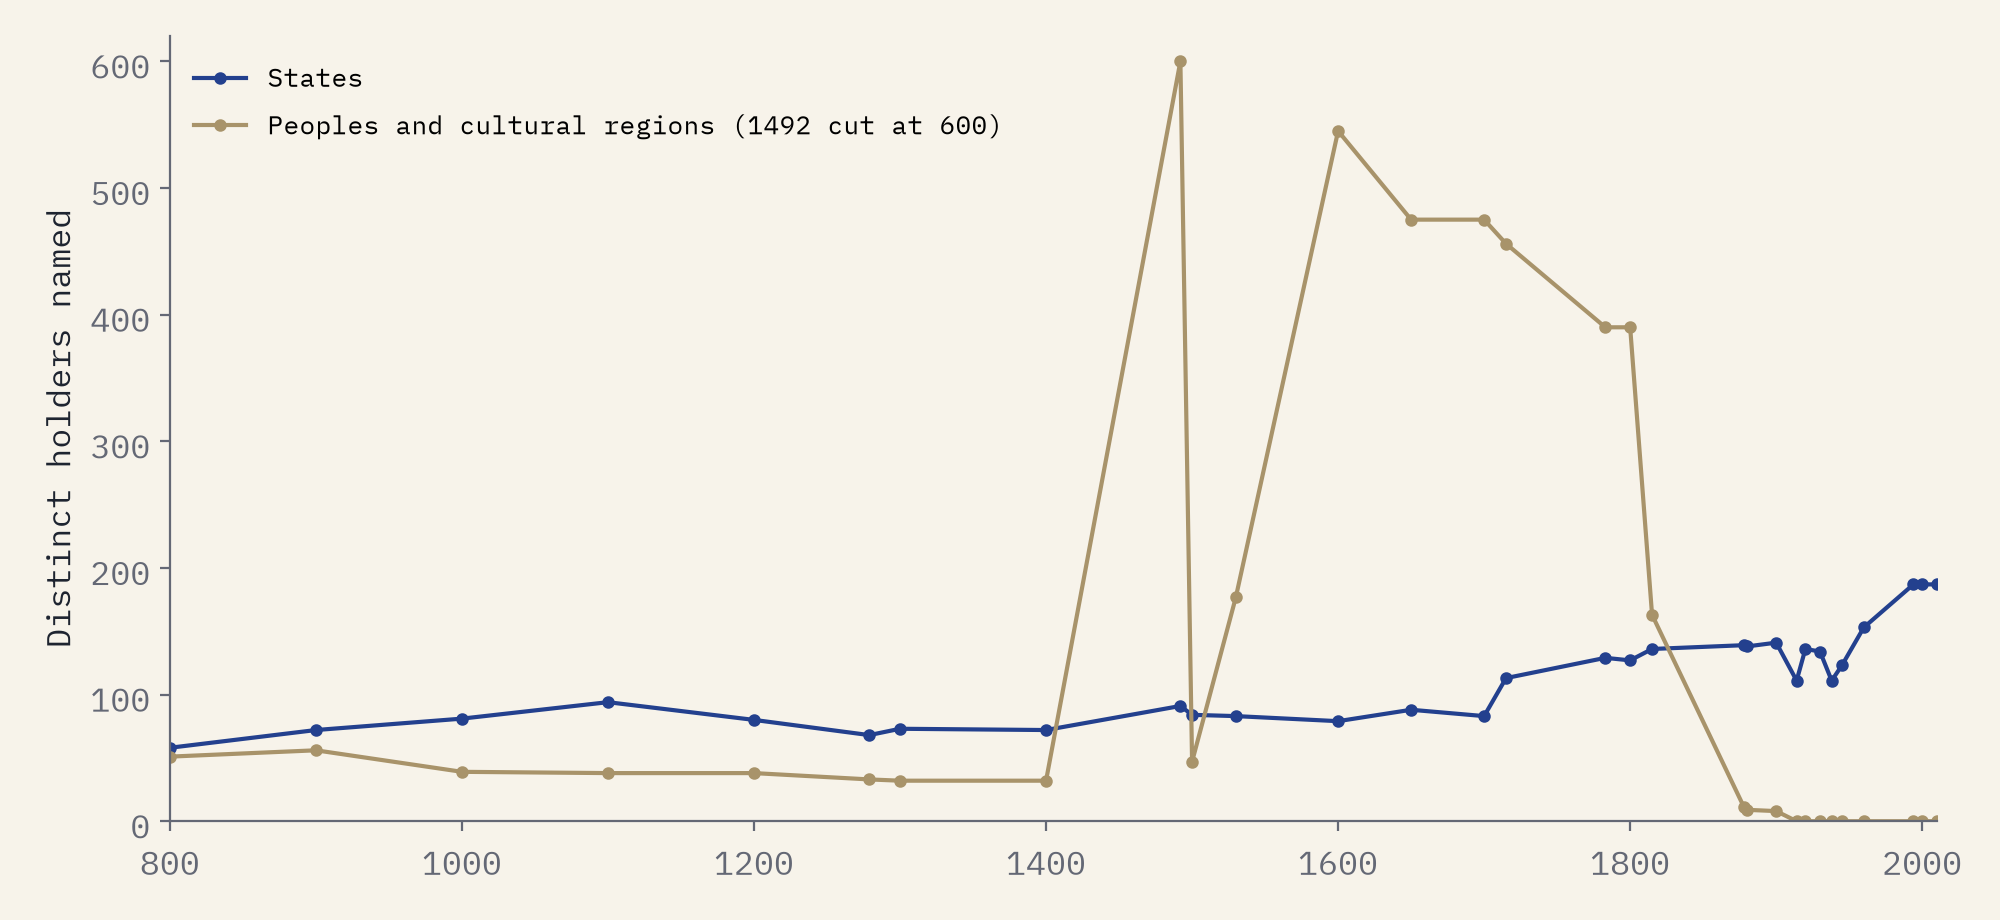
\includegraphics[width=.86\textwidth]{f_states.png}
\caption{Distinct states and peoples or cultural regions named in each snapshot.}\label{fig:states}\end{figure}

\subsection{The age of today's flags}
Wikidata gives a start date for the current flag of 93 of 194 present-day countries (48\%\%; Figure~\ref{fig:age}). The busiest period is 1980 to 1999 (26 countries), and the median is 1986. Many dates are of a version rather than a design (Japan 1999, Italy 2006, France 2020), and long-established flags without dates, such as Denmark's, are missing, so the chart should not be read as the age of the designs.

\begin{figure}[tbp]\centering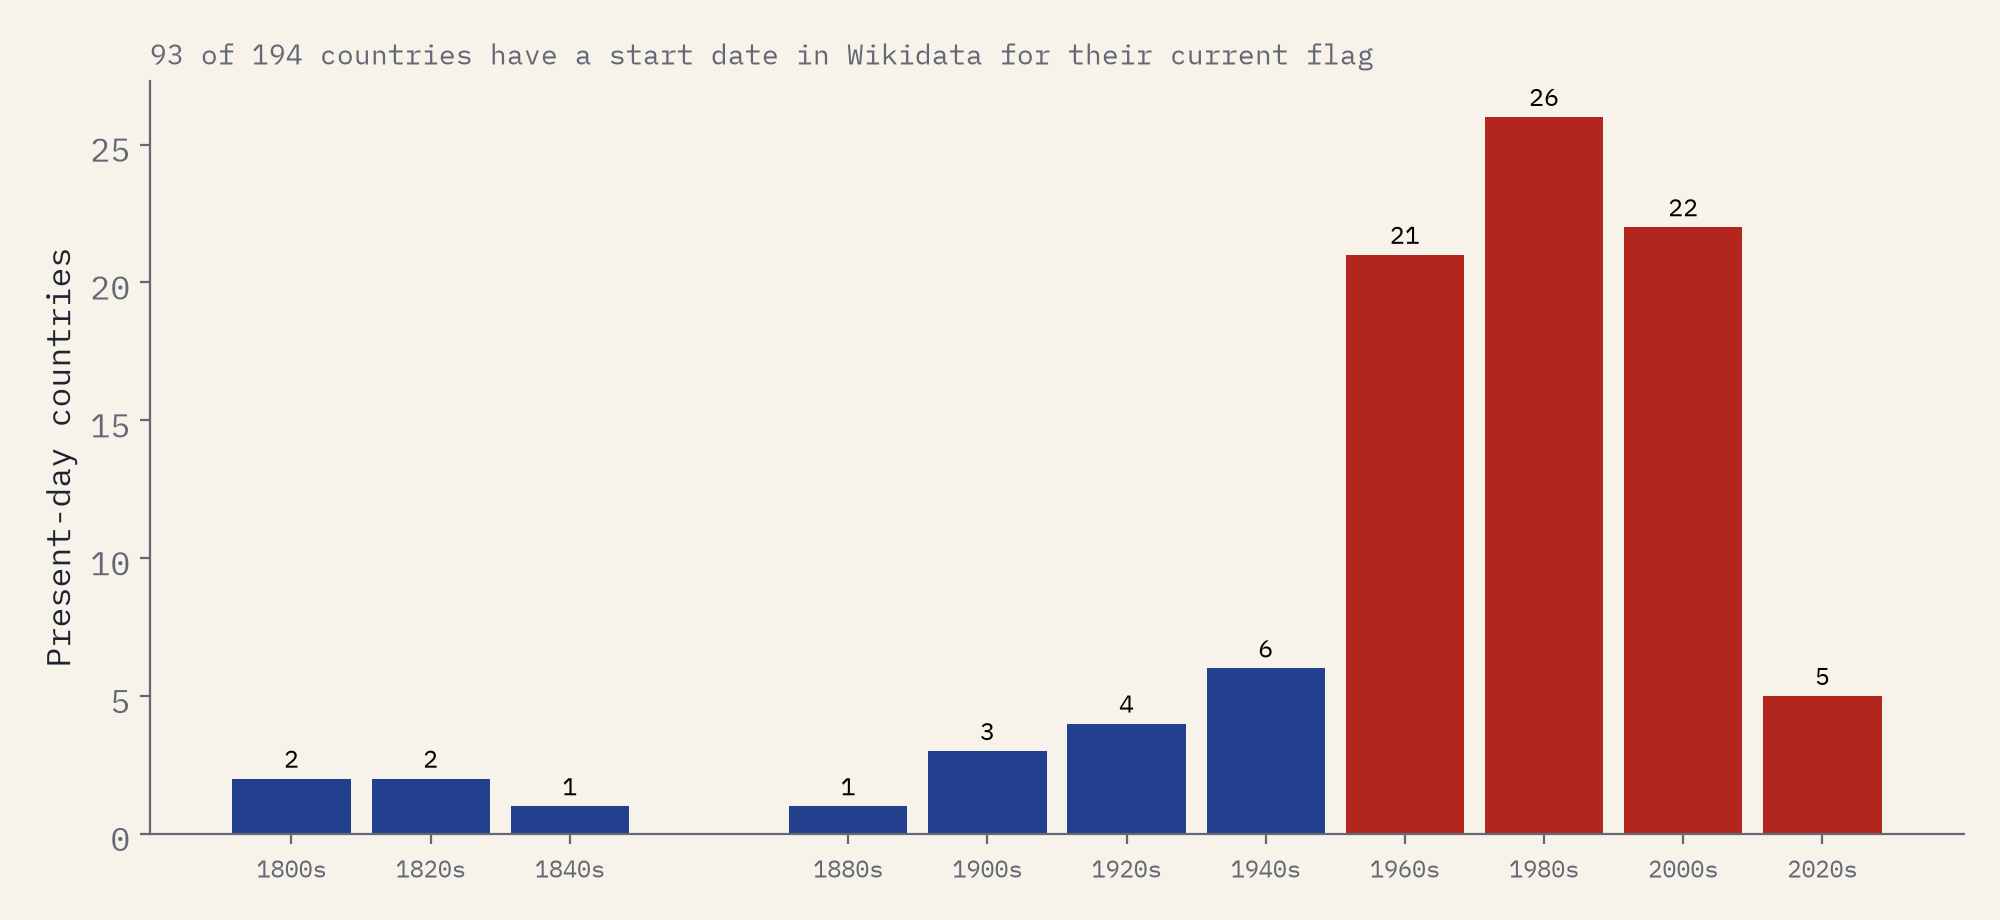
\includegraphics[width=.86\textwidth]{f_age.png}
\caption{Start year of each present-day country's current flag in Wikidata, by 20-year period.}\label{fig:age}\end{figure}

\section{Limitations}
First, the basemaps are simplified and in places wrong or disputed; borders before 1500 are guesses at frontiers that were often zones, and a single holder hides vassals, tribute and shared rule. Second, the level of detail varies between snapshots, which affects counts. Third, flags depend on what Wikidata records: well-documented states are rich in flags, others have none, so the map shows the reach of the record as well as of flags. Fourth, 42\%\% of flags shown rest on undated statements and may be shown a few years early. Fifth, name matching is automatic for most holders; I checked the largest by hand, but some small ones will have matched a namesake. Sixth, the European share uses representative points to place areas in or outside Europe.

\section{Conclusion}
A world map in flags is easy to draw for 2010 and impossible to draw honestly for 1000. Between the two, the map fills as national flags spread from ships to states and from Europe across its empires. The rules here make each choice visible, and the interactive version lets readers check any area, its flag and its source.

\section*{Data and code availability}
The interactive map is at \url{https://maps.tristanhotham.com/flags-through-time/}. Data and code are at \url{https://github.com/Tristan-Hotham/flags-through-time} and archived with this paper at \url{https://doi.org/10.5281/zenodo.23845995}. The simplified boundaries and area tables derive from historical-basemaps and are released under GPL-3.0; flag images keep their own licences (listed in data/flag\_credits.csv); the text and figures are CC BY-SA 4.0 because some flag images are CC BY-SA; code is MIT.

\section*{AI statement}
I wrote the text, with drafting and editing assistance from Claude (Anthropic), which also helped prepare the analysis code. I reviewed and checked all text and results.

\begin{thebibliography}{9}
\bibitem[Lipiridis(2026)]{flagicons} Lipiridis, P. (2026) flag-icons. MIT licence. \url{https://github.com/lipis/flag-icons}
\bibitem[Natural Earth(2026)]{naturalearth} Natural Earth (2026) Admin 0 countries and populated places. Public domain. \url{https://www.naturalearthdata.com/}
\bibitem[Ourednik(2026)]{ourednik} Ourednik, A. and contributors (2026) historical-basemaps: historical boundaries of world countries and cultural regions. GPL-3.0. \url{https://github.com/aourednik/historical-basemaps}
\bibitem[Pastoureau(1997)]{pastoureau} Pastoureau, M. (1997) \emph{Heraldry: its origins and meaning}. London: Thames and Hudson.
\bibitem[QLever(2026)]{qlever} Bast, H. and Buchhold, B. QLever SPARQL engine, Wikidata endpoint. \url{https://qlever.cs.uni-freiburg.de/wikidata}
\bibitem[Vrande\v{c}i\'c and Kr\"otzsch(2014)]{wikidata} Vrande\v{c}i\'c, D. and Kr\"otzsch, M. (2014) Wikidata: a free collaborative knowledgebase. \emph{Communications of the ACM}, 57(10), 78 to 85.
\end{thebibliography}
\end{document}
